\documentclass[twocolumn,showpacs,preprintnumbers,amsmath,amssymb,prb]{revtex4}
\usepackage{graphicx,amssymb,amsmath}
\usepackage[usenames]{xcolor}
\newcommand{\etalter}{{\it et al.}}
\newcommand{\eg}{{\it e.\ g.}}
\newcommand{\ie}{{\it i.\ e.}}

\begin{document}

\title{Title goes here}
\author{G. A.}
\affiliation{ORNL}

\begin{abstract}
Here goes the abstract....
\end{abstract}

\maketitle

Definition: Consider a MERA $|\psi\rangle$ with $N$ free indices of
\emph{arity} (or \emph{ary}) $a$ and dimension $d$, and let us label $T_0$, $T_1$, \ldots, $T_X$, 
 all tensors constituting the MERA
$|\psi\rangle$. Picture MERA as a pyramid in Figure 1(a).

Definition: A Hamiltonian $H$ is a tensor of $2N$ indices that act on $|\psi\rangle$ and yields
a $N$-index tensor $H|\psi\rangle$. $H$ is symmetric, meaning, invariant under the swapping of the first
and last $N$ indices. (More generally, $H$ is Hermitian, meaning, that it needs complex conjugation
after the swapping to remain invariant.) 
Although not essential, we will work mostly with local Hamiltonians so the following definition will
become useful at some point.

Definition: A Hamiltonian $H$ is $k-$local if it can be written as a sum of (at most) $k$-index tensors:
$H=\sum_l H_l$ where each $H_l$ is of rank (at most) $k$.

Definition: Given $H$, the energy of the MERA $|\psi\rangle$ is the scalar $E(|\psi\rangle)\equiv \langle \psi | H |\psi\rangle$,
which is real because $H$ is Hermitian. Picture $E$ as a diamond, with an upper MERA and a lower conjugated MERA, and
$H$ in between, as in Figure 1(b).

The Problem: Find the\footnote{Existence and uniqueness is left as an exercise to the reader.} 
MERA $|\psi\rangle$ that minimizes the energy functional
$E(|\psi\rangle)\equiv \langle \psi | H |\psi\rangle$, where $H$ is a given local Hamiltonian.

The solution: (Algorithm follows.) 
Consider $E$ as a function of \emph{only} tensor $T_0$ with the other tensors $T_i$ $i>0$ fixed
and taking random values.
That is, we want to minimize the functional $E(T_0)$ with all other tensors fixed. Unfortunately, 
 $T_0$ appears both in the upper part of the diamond $E$, and in the lower part in conjugated form $T_0^*$.
\emph{Fill} the lower $T_0^*$ with random values so that $E(T_0)$ depends on $T_0$ only in the upper part of $E$.
For some known $B_0$, one can then write $E(T_0) = \textrm{Tr}(T_0 B_0)$.
$B_0$ can be visualized as $E$ with a hole where the upper $T_0$ was. That is, $B_0$ is the tensor that results
from deleting the upper $T_0$ from the diamond $E$, as in Figure 1(c).
Using the Lemma below, \emph{do} an SVD decomposition of $B_0 = USV^\dagger$, and obtain $T_0$ as $-VU^\dagger$.
Replace this found $T_0$ and also $T_0^*$ into their places in the diamond $E$ and proceed to tensor $T_1$.
Now consider $E(T_1)$ as a function of \emph{only} $T_1$, with $T_0$ computed before, and with $T_i$, $i > 1$
taking
the random values set up at the beginning. Minimize $E$ as a function of $T_1$ only, as follows.
For some known $B_1$, one can then write $E(T_1) = \textrm{Tr}(T_1 B_1)$. 
Using the Lemma below, \emph{do} an SVD decomposition of $B_1$ to obtain $T_1$ as before.
Repeat this process for $T_2$, $T_3$, \ldots, until all tensor are computed. Start again from the beginning and proceed over and over until
convergence. Now instead of random values, you
have the computed values for each $T_i$.
For simplicity, this description doesn't take into account caching, but caching is of paramount importance
for performance. It also doesn't describe causal cone simplifications. And finally, it doesn't constrain the
minimization to any symmetry.\footnote{Of these three \emph{complications}, only causal cone simplifications are
	implemented in MERA++.}
\begin{figure}[b]
	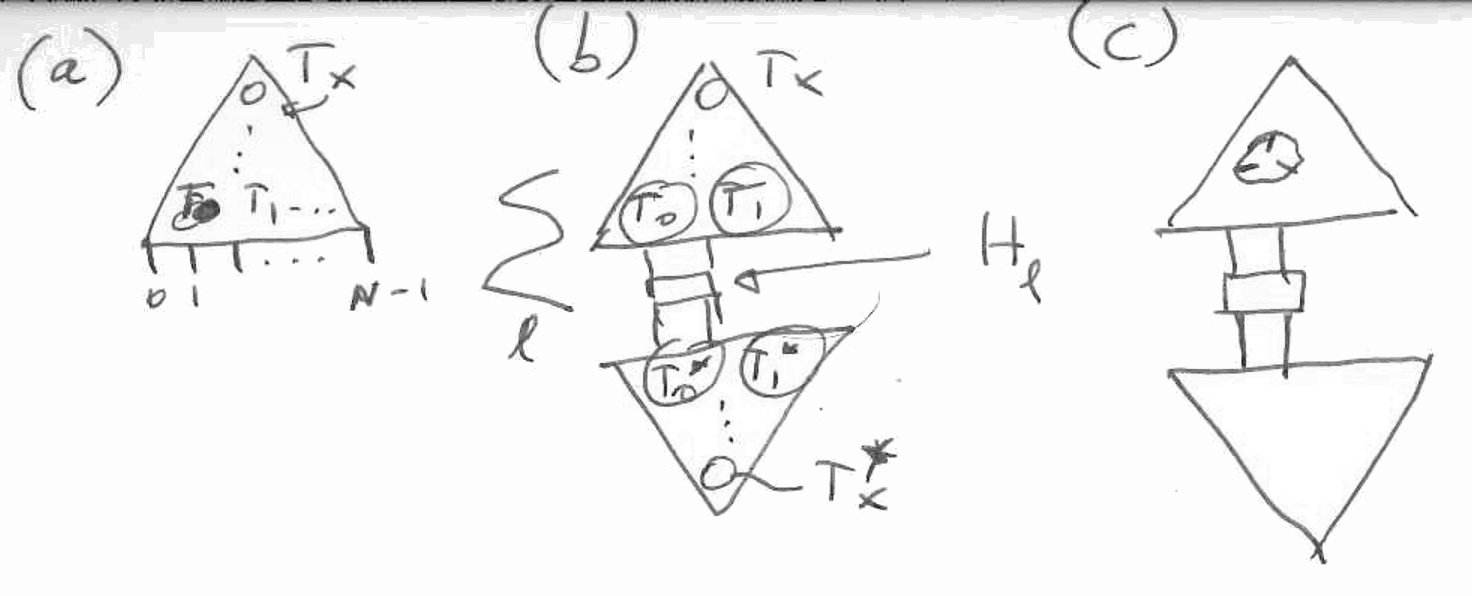
\includegraphics[width=0.45\textwidth]{figure.png}
	\caption{(a) A MERA with $N$ free indices and tensor $T_0$, $T_1$, \ldots, $T_X$. 
		(b) The scalar $E(|\psi\rangle)\equiv \sum_l\langle \psi | H_l |\psi\rangle$ pictured for only one $l$.
		(c) The tensor $B_0$ formed by deleting the tensor $T_0$ from the upper MERA of $E$. In the resulting hole, the
		free indices of $B_0$ are pictured.}
\end{figure}

Lemma:
Let $E(A) = Tr(AB)$ and $B = USV^\dagger$ the svd decomposition of $B$.
Then minimum of $E$ with respect to $A$ under the condition that $A^\dagger A = I$
is realized for $A = -VU^\dagger.$


Proof: 
\begin{align}
E(A) = Tr(AB) =& Tr(AUSV^\dagger)\nonumber\\
 =& Tr(V^\dagger A U S) = Tr(\bar{A} S)
\label{eq:trace}
\end{align}
where $\bar{A} \equiv V^\dagger A U.$  Then $\bar{A}^\dagger \bar{A} = I$ or
$\sum_k \bar{A}^*_{k,i}\bar{A}_{k,j} = \delta_{i,j}$ for all $i,j$.
$\sum_k |\bar{A}_{k,i}|^2 = 1$ for all $i$ or
$|\bar{A}_{i,i}|^2 + \sum_{k\neq i} |\bar{A}_{k,i}|^2 = 1$ for all $i$ or
$|\bar{A}_{i,i}| <= 1$ for all $i$ or
$\bar{A}_{i,i} >= -1$ for all $i$.
Then 
\begin{equation}
E(A) = Tr(\bar{A} S) = \sum_i \bar{A}_{i,i} S_i \le -\sum_i S_i
\end{equation}
because $S_i \ge 0$ for all $i$.
The minimum is realized if $\bar{A}_{i,i} = -1$ for all $i$, and 
from Eq.~(\ref{eq:trace}) we get
then $|\bar{A}_{k,i}|^2 = 0$ for all $k\neq i$,
implying $\bar{A}_{k,i} = 0$ for all $k\neq i$
Then $\bar{A} = -I$, implying $V^\dagger A U = -I$, from which the end result follows.
\end{document}